\Answer{}
The problem to solve is
%
\begin{spreadlines}{2ex} % See https://tex.stackexchange.com/a/577172
    \begin{equation}
        \begin{dcases}
            \begin{aligned}
                \nabla^2 \phi(x, y) & = -\rho, & (x, y) \in \square;         \\
                \phi(x, y)          & = 0,     & (x, y) \in \partial\square; \\
                \phi(x, y)          & = 5,     & (x, y) \in \blacksquare;
            \end{aligned}
        \end{dcases}
    \end{equation}
\end{spreadlines}
%
where \(\square\) denotes the two-dimensional simulation box,
\(\partial\square\) denotes the boundary of the box,
and \(\blacksquare\) denotes the solid internal square.

% % See https://tex.stackexchange.com/a/227247
\begin{figure}
    \centering
    \begin{tikzpicture}
        \draw[thick] (0,0) grid (4,4); % See https://tex.stackexchange.com/a/552215
        \stencilpt[red]{2,2}{i}  {$-4$};
        \stencilpt{1,2}{i-1}{$1$};
        \stencilpt{3,2}{i+1}{$1$};
        \stencilpt{2,1}{j-1}{$1$};
        \stencilpt{2,3}{j+1}{$1$};
        \draw
        (j-1) -- (i)
        (i)   -- (j+1)
        (i-1) -- (i)
        (i)   -- (i+1);
    \end{tikzpicture}
    \caption{The \href{https://en.wikipedia.org/wiki/Five-point_stencil}{five-point stencil}
        for the discretization of a Laplacian using central differences.}
    \label{fig:stencil}
\end{figure}


First, we want to discretize the Laplacian operator \(\nabla^2\).
With grid spacing \(a\), the standard discretization for a square grid is
%
\begin{equation}\label{eq:del2phi}
    \nabla^2 \phi(x, y) =
    \frac{ 1 }{ a^2 } \bigl(\phi(x - a, y) - 2 \phi(x, y) + \phi(x + a, y)\bigr) +
    \frac{ 1 }{ a^2 } \bigl(\phi(x, y - a) - 2 \phi(x, y) + \phi(x, y + a)\bigr).
\end{equation}
%
We simplify Equation~\eqref{eq:del2phi} as
%
\begin{equation}\label{eq:del2phisim}
    \bigl(\nabla^2 \phi\bigr)_{i, j} = \frac{1}{a^2} \bigl(
    -4 \phi_{i, j} + \phi_{i+1, j} + \phi_{i-1, j} + \phi_{i, j-1} + \phi_{i, j+1}
    \bigr),
\end{equation}
%
for all \(i\) and \(j\),
where \(i\) and \(j\) label the \(x\) and \(y\) coordinates, respectively.
By starting at the lower left corner and traversing in the \(y\)-direction first, and
subsequently in the \(x\)-direction---the lexicographical ordering---we get the following
system of equations:
%
\begin{align}
    \bigl(\nabla^2 \phi\bigr)_{i, j+1}   & = \frac{1}{a^2} (
    \phi_{i, j} - 4\phi_{i, j+1} + \phi_{i, j+2} + \phi_{i+1, j+1} + \phi_{i-1, j+1}
    ),                                                       \\
    \bigl(\nabla^2 \phi\bigr)_{i+1, j}   & = \frac{1}{a^2} (
    \phi_{i, j} - 4\phi_{i+1, j} + \phi_{i+1, j+1} + \phi_{i+1, j-1} + \phi_{i+2, j}
    ),                                                       \\
    \bigl(\nabla^2 \phi\bigr)_{i+1, j+1} & = \frac{1}{a^2} (
    \phi_{i, j+1} + \phi_{i+1, j} - 4\phi_{i+1, j+1} + \phi_{i+1, j+2} + \phi_{i+2, j+1}
    ),                                                       \\
    \shortvdotswithin{=} % See https://tex.stackexchange.com/a/67196
    \bigl(\nabla^2 \phi\bigr)_{i-1, j-2} & = \frac{1}{a^2} (
    \phi_{i-1, j-3} + \phi_{i, j-2} + \phi_{i-2, j-2} - 4\phi_{i-1, j-2} + \phi_{i-1, j-1}
    ),                                                       \\
    \bigl(\nabla^2 \phi\bigr)_{i-1, j-1} & = \frac{1}{a^2} (
    \phi_{i-1, j} + \phi_{i-1, j-2} + \phi_{i, j-1} + \phi_{i-2, j-1} - 4\phi_{i-1, j-1}
    ).\label{eq:delend}
\end{align}
%
Here we apply the periodic boundary condition
%
\begin{align}
    \phi(x + (N-1)a, y) & = \phi(x - a, y), \\
    \phi(x, y + (N-1)a) & = \phi(x, y - a).
\end{align}

\begin{figure}
    \centering
    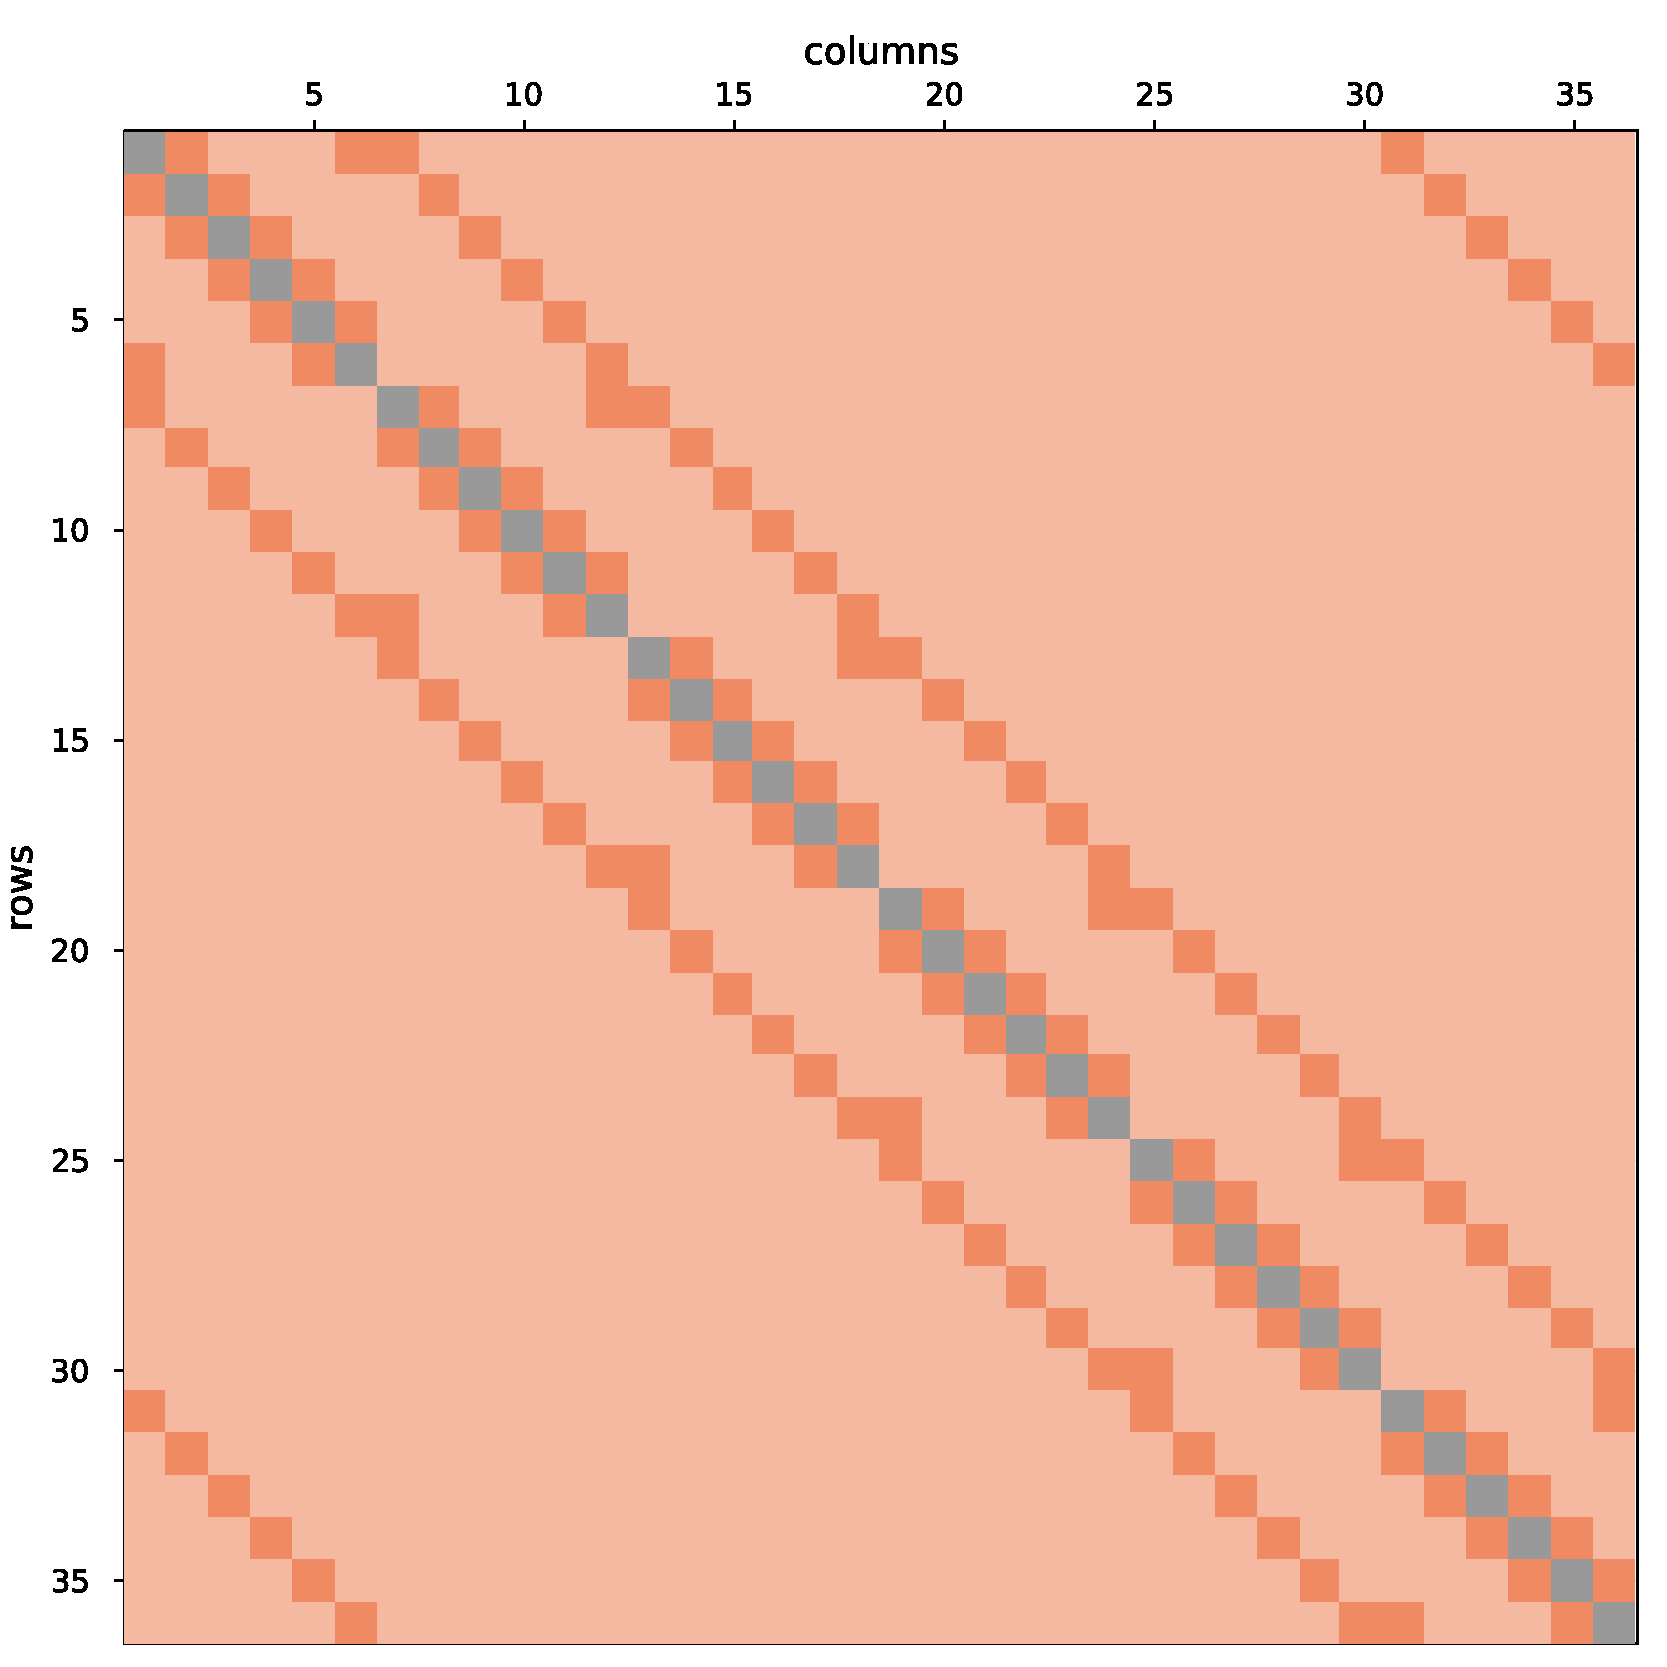
\includegraphics[width=0.8\textwidth]{laplacian}
    \caption{The heatmap of the discrete Laplacian with \(N = 32\), and hence
        the Laplacian matrix is of size \(1024 \times 1024\).
        The color red denotes the terms \(-4\) on the diagonal of the matrix, and
        the color dark gray denotes the ones, and the background gray
        denotes the zeros.
        As we can observe, the discrete Laplacian is a sparse matrix.}
    \label{fig:laplacian}
\end{figure}

We can simplify Equations~\eqref{eq:del2phisim} to~\eqref{eq:delend} into a matrix
representation, i.e., the discrete Laplacian representation:
%
\begin{equation}\label{eq:Axb}
    \begin{split}
        -\bm{\rho} &= \frac{ 1 }{ a^2 } \begin{bsmallmatrix}
            -4     & 1      & 0      & \cdots & 0      & 1      & 1      & 0      & \cdots & 0      & 0      & \cdots & 1      & \cdots & 0      & 0      \\
            1      & -4     & 1      & \cdots & 0      & 0      & 0      & 1      & \cdots & 1      & 0      & \cdots & 0      & \cdots & 0      & 0      \\
            \vdots & \vdots & \vdots & \ddots & \vdots & \vdots & \vdots & \vdots & \ddots & \vdots & \vdots & \ddots & \vdots & \ddots & \vdots & \vdots \\
            1      & 0      & 0      & \cdots & 0      & 0      & -4     & 1      & \cdots & 1      & 1      & \cdots & 0      & \cdots & 0      & 0      \\
            0      & 1      & 0      & \cdots & 0      & 0      & 1      & -4     & \cdots & 0      & 0      & \cdots & 0      & \cdots & 0      & 0      \\
            \vdots & \vdots & \vdots & \ddots & \vdots & \vdots & \vdots & \vdots & \ddots & \vdots & \vdots & \ddots & \vdots & \ddots & \vdots & \vdots \\
            0      & 0      & 0      & \cdots & 1      & 0      & 0      & 0      & \cdots & 0      & 0      & \cdots & 0      & \cdots & -4     & 1      \\
            0      & 0      & 0      & \cdots & 0      & 1      & 0      & 0      & \cdots & 0      & 0      & \cdots & 1      & \cdots & 1      & -4
        \end{bsmallmatrix}
        \begin{bsmallmatrix}
            \phi_{0, 0} \\
            \phi_{0, 1} \\
            \phi_{0, 2} \\
            \vdots \\
            \phi_{0, N-2} = \phi_{0, -2} \\
            \phi_{0, N-1} = \phi_{0, -1} \\
            \phi_{1, 0} \\
            \phi_{1, 1} \\
            \vdots \\
            \phi_{1, N-1} = \phi_{1, -1} \\
            \phi_{2, 0} \\
            \vdots \\
            \phi_{N-1, 0} = \phi_{-1, 0} \\
            \vdots \\
            \phi_{N-1, N-2} = \phi_{-1, -2} \\
            \phi_{N-1, N-1} = \phi_{-1, -1}
        \end{bsmallmatrix} \\
        &= \mathrm{ A } \bm{\phi},
    \end{split}
\end{equation}
%
where \(\mathrm{ A }\) (the discrete Laplacian) is a \(N^2 \times N^2\) matrix,
and \(\bm{\phi}\) and \(\bm{\rho}\) are \(N^2 \times 1\) vectors.
Notice that the structure of the coefficient matrix \(\mathrm{ A }\) is completely dictated
by the way that the basis is ordered.
The non-zero elements in the coefficient matrix are markers for which \(\phi\) is coupled
with each other.
The heatmap of a discrete Laplacian with \(N = 32\) is plotted in Figure~\ref{fig:laplacian}.
The corresponding Laplacian matrix is of size \(1024 \times 1024\).
Obviously, the discrete Laplacian is a sparse matrix.
We could use sparse matrix algorithms or just use~\eqref{eq:del2phi} in the actual
implementation.
In vector \(\bm{\phi}\), we order the \(\phi\)'s in \(y\)-direction first and then
\(x\)-direction, as stated above.

For a box of size \(N\), the linear index \(n\) of point \((i, j)\) on the grid is
%
\begin{equation}\label{eq:nij}
    n = N i + j,
\end{equation}
%
in the \(y\)-direction first indexing order, where \(n = 1\), \(\ldots\), \(N^2\).
And since \(x = a i = i\), \(y = a j = j\),~\eqref{eq:nij} can be rewritten as
%
\begin{equation}
    n = N x + y.
\end{equation}
%
We draw a schematic plot of the system with \(N = 32\) for simplicity in
Figure~\ref{fig:grid}, where you can observe this relation.
In the iterative solver for Equation~\ref{eq:Axb},
the initial vector \(\bm{\rho}(0)\) has \(\rho(0)_a = -20\) and \(\rho(0)_b = -20\),
and zero everywhere else,
where \(a\) and \(b\) are the linear indices of the two charges.
And the initial vector \(\bm{\phi}(0)\) has \(5\) in the components corresponding to
the points in the solid square, and has zero in the components corresponding to
the boundary of the region while having non-zero values everywhere else.
The solid square in the interior has length \(\frac{1}{4}\) and height \(\frac{1}{4}\) and
its center is at \((x, y) = (\frac{5}{8}, \frac{3}{4})\).
The point charges are at \((\frac{1}{4}, \frac{1}{8})\) and \((\frac{3}{4}, \frac{1}{8})\).
